\originalchapter{15.053 期中2综合练习}\label{ass:15053-practice}
本章对应 OCW 网页归类的 Midterm Exam 2 practice problem set. PDF 本身标题为 \emph{Practical Problem Set, 2013}, 是综合练习, 不能当作已经公开的正式期中试卷. 原编号为1、2、3、4、5、5, 后两题在本章映射为5(a)、5(b). 题面 PDF 的九报价版本与官方解答 PDF 的七报价旧版本不同, 下文完整保留题面版本, 注明答案的版本差异和 AI 补解.

\begin{exercise}\label{ass:15053-practice-q1}
原题1. 组合拍卖允许对一整组物品报价, 每份报价不可拆分. 有六种物品 $\{1,2,3,4,5,6\}$, 收到下列九份报价:
\begin{center}\begin{tabular}{c|l|r}报价 $j$&物品集合 $S_j$&总价 $p_j$\\\hline
1&$\{1,5\}$&10\\2&$\{1,2,4\}$&20\\3&$\{3\}$&8\\4&$\{5\}$&4\\5&$\{2,4\}$&15\\6&$\{2,3,4,5\}$&30\\7&$\{1,2,3\}$&18\\8&$\{2,4,6\}$&25\\9&$\{3,5,6\}$&16
\end{tabular}\end{center}
\begin{enumerate}[label=(\alph*)]
\item 每物品最多卖一次, 建使拍卖收入最大的整数规划, 仅用二元 $x_j$ 表示接受报价 $j$.
\item 物品1、2、3各有两份, 4、5、6各一份, 即多重集 $\{1,1,2,2,3,3,4,5,6\}$. 各报价仍只能接受一次, 修改模型. 原文上一句仍写“$\{1,\ldots,5\}$”, 与明确多重集和报价8、9不一致, 此处以列出的多重集为准.
\item 一般物品集合 $N=\{1,\ldots,n\}$, 每物品 $i$ 有 $\lambda_i\ge1$ 份, 有 $b$ 报价 $(S_j,p_j)$, 写代数模型.
\end{enumerate}
\end{exercise}
\begin{solution}
官方通用结构重构, 九报价实例由 AI 独立补解. (a) 最大化 $10x_1+20x_2+8x_3+4x_4+15x_5+30x_6+18x_7+25x_8+16x_9$, 所有 $x_j\in\{0,1\}$, 六条约束为
\[
\begin{aligned}
x_1+x_2+x_7&\le1,&x_2+x_5+x_6+x_7+x_8&\le1,\\
x_3+x_6+x_7+x_9&\le1,&x_2+x_5+x_6+x_8&\le1,\\
x_1+x_4+x_6+x_9&\le1,&x_8+x_9&\le1.
\end{aligned}
\]
每条限制同一物品不会被重复出售, 二元变量确保报价整体接受. (b) 只把前三条 RHS 改2, 后三条仍1; 二元域仍保留, 不允许同一报价接受两次. (c) 通式为 $\max\sum_{j=1}^bp_jx_j$, $\sum_{j:i\in S_j}x_j\le\lambda_i$（每个 $i$）, $x_j\in\{0,1\}$.

实际枚举全部 $2^9=512$ 组合核验: (a) 接受1、3、8, 收入43; (b) 接受1、3、7、8, 收入61, 两者均为唯一最优组合. 官方答案只列前七报价、五物品模型, 不能直接声称覆盖本题九报价版本; 其通式仍可用于新版本.
\end{solution}

\begin{exercise}\label{ass:15053-practice-q2}
原题2（模型数据独立重述）. 课程引用 Cornu\'{e}jols 与 T\"ut\"unc\"u 的 \emph{Optimization Methods in Finance} 的收款箱例, 这里只重述给定数学数据, 不转载外书叙述. 四地区西部、中西部、东部、南部每天收款分别600000、250000、725000、350000美元. 候选收款箱依次为 Los Angeles、Chicago、Boston、Houston, 每箱年运营费90000美元, 总部 Seattle 可免费处理. 五目的地的平均清算天数为
\[
D=\begin{pmatrix}2&4&6&6&5\\4&2&5&5&4\\6&5&2&5&7\\7&5&6&3&9\end{pmatrix}.
\]
资金年利率4\%, 年机会成本（千美元） $C_{ij}=0.04\,a_iD_{ij}/1000$, 即
\[
C=\begin{pmatrix}48&96&144&144&120\\40&20&50&50&40\\174&145&58&145&203\\98&70&84&42&126\end{pmatrix}.
\]
令 $y_j=1$ 表示候选箱 $j$ 开设（$j=1,\ldots,4$）, $x_{ij}=1$ 表示地区 $i$ 向目的地 $j$ 寄送（$j=1,\ldots,5$, 5是 Seattle）.
\begin{enumerate}[label=(\alph*)]
\item 写包含开箱和延迟机会成本的目标函数.
\item 写禁止向未开箱寄送的约束, 共多少条?
\item 写每地区目的地分配约束.
\item 汇总完整模型, 还有哪些条件必须补上?
\item 给(b)的另一种表达. 原文误引用“Problem 3.b”, 应按本题(b)理解.
\item 开三个或四个候选箱时另加50000美元年费, 不计 Seattle. 建模并说明目标如何变.
\end{enumerate}
\end{exercise}
\begin{solution}
官方结构重构, AI 修正其汇总模型的连接约束. (a) 以千美元计, $\min90\sum_{j=1}^4y_j+\sum_{i=1}^4\sum_{j=1}^5C_{ij}x_{ij}$. 延迟导致的在途资金为“每日金额乘天数”, 再乘年利率, 不再额外乘365.

(b) $x_{ij}\le y_j$（$i=1,\ldots,4$, $j=1,\ldots,4$）, 共16条; Seattle 不受开箱限制. (c) $\sum_{j=1}^5x_{ij}=1$（每个 $i$）, 共4条. (d) 合并上述目标与20条约束, 补全 $x_{ij},y_j\in\{0,1\}$. (e) 可替为 $\sum_{i=1}^4x_{ij}\le4y_j$（每个候选箱 $j$）, 共4条. 由于二元变量, 箱关闭时四个分配都为0, 箱开时最多四地区, 与16条版本在整数点上等价. 官方汇总式漏乘4, 写成 $\sum_i x_{ij}\le y_j$, 会错误禁止两个地区共用同一箱. 16条版本的连续松弛通常更强.

(f) 二元 $w$, $\sum_jy_j\le2+2w$, 目标加 $50w$. 在极小目标下 $w$ 只在开三或四箱时取1, 足以保证最优方案计费正确. 若要求每个可行点也精确记录是否收费, 再加 $3w\le\sum_jy_j$.

附带脚本枚举16种开箱组合并对每地区选最低成本允许目的地: 最优只开 Boston, 西部、中西部发 Seattle, 东部、南部发 Boston, 年成本 $90+120+40+58+84=392$千美元. 加额外年费后方案仍相同. 这也是对“每箱可服务多地区”的实际验算.
\end{solution}

\begin{exercise}\label{ass:15053-practice-q3}
原题3. 选择所有适用选项.
\begin{enumerate}[label=(\alph*)]
\item 原整数集 $P$ 为 $x/2+y\le1$, $2x+y\le2$, $x,y\le0$, $x,y\in\mathbb Z$. 它与下列哪项等价? (i) $x+y\le1$, $x,y$ 整数; (ii) $x\le1,y\le1$, $x,y$ 整数; (iii) 两者; (iv) 两者都不是.
\item 极大整数规划与其 LP 松弛, 在最优值存在的相应情形记 $Z_{\mathrm{IP}},Z_{\mathrm{LP}}$. 哪些可能? (i) IP 不可行而 LP 可行; (ii) IP 可行而 LP 不可行; (iii) $Z_{\mathrm{IP}}=Z_{\mathrm{LP}}$; (iv) $Z_{\mathrm{IP}}>Z_{\mathrm{LP}}$; (v) $Z_{\mathrm{IP}}<Z_{\mathrm{LP}}$.
\item 对极大 LP 松弛添加有效 Gomory 割, 最优值记 $Z_{\mathrm{GC}}$, 假定两个最优值都存在. 哪些可能? (i) $Z_{\mathrm{LP}}=Z_{\mathrm{GC}}$; (ii) $Z_{\mathrm{LP}}>Z_{\mathrm{GC}}$; (iii) $Z_{\mathrm{LP}}<Z_{\mathrm{GC}}$.
\item 极大0--1规划分支树节点 $v$ 的有限松弛值为 $\mathrm{LP}(v)$, 子节点 $c_1,c_2$ 对某二元变量取0、1. 哪些可能? (i) 两子松弛都不可行; (ii) $\mathrm{LP}(v)=\mathrm{LP}(c_1)$; (iii) $\mathrm{LP}(v)>\max\{\mathrm{LP}(c_1),\mathrm{LP}(c_2)\}$; (iv) $\mathrm{LP}(v)<\min\{\mathrm{LP}(c_1),\mathrm{LP}(c_2)\}$.
\end{enumerate}
\end{exercise}
\begin{solution}
(a) AI 修正原符号条件下的官方答案. 原条件 $x,y\le0$ 使两斜约束自动满足, 所以 $P$ 恰为非正整数象限. 选(iv): (i)还含 $(2,-1)$, (ii)还含 $(1,1)$, 均不等于 $P$. 官方选(i), 显然未按原显示的非正条件处理. 若\textbf{另行修正}原条件为 $x,y\ge0$ 并且在选项(i)补同样的非负域, 则三个点 $(0,0),(1,0),(0,1)$ 恰满足(i); 这是一份条件不同的 AI 解释版本, 不能替代原题.

(b) 官方答案重构: 选(i)、(iii)、(v). 整数点集合是 LP 集合子集, 因此(ii)、(iv)不可能. 约束 $x=1/2,x\in\mathbb Z$ 示(i); 最大化 $x$, $0\le x\le1$ 示(iii); 将上界改1/2示(v).

(c) 官方答案重构: 选(i)、(ii). 加有效割只缩小松弛可行集, 不能提高极大值. 恒零目标可保持相同值; $\max x$, $0\le x\le1/2$ 加整数割 $x\le0$ 可严格下降.

(d) 官方答案重构: 选(i)、(ii)、(iii). 父约束 $x=1/2$ 可使两子都不可行; $\max x$, $0\le x\le1$ 在子 $x=1$ 保持值1. 对二元 $x,t$ 加 $t\le x,t\le1-x$, 最大化 $t$, 根松弛 $(x,t)=(1/2,1/2)$ 值1/2, 两子都只能 $t=0$, 示(iii). 子集关系排除(iv). 比较两个子值时, 不可行子可用$-\infty$作为极大值约定.
\end{solution}

\begin{exercise}\label{ass:15053-practice-q4}
原题4.
\begin{enumerate}[label=(\alph*)]
\item 用整数规划表示“$x_1+x_2+x_3+x_4\le4$ 或 $3x_1-x_2-x_3+x_4\le3$ 至少一条成立”. 原题面未给变量上下界; 官方答案另加 $x_j\ge0$ 整数, 但仍无上界.
\item $f(y)=10y$（整数 $0\le y\le50$）, $500$（$51\le y\le100$）, $5y$（$y\ge101$）. 将
\[
\min\ f(x_1)+6x_2,\qquad1001x_1+978x_2\le27365,\qquad503x_1+631x_2\le16783,\qquad x_1,x_2\text{整数}
\]
改写为整数规划. 原题未给非负约束, 且 $f$ 未定义在负整数上.
\end{enumerate}
\end{exercise}
\begin{solution}
AI 保留原条件缺口并给明确模型版本. (a) 令二元 $w$, 原逻辑可直接交给支持指示约束的整数求解器:
$w=0\Rightarrow\sum_jx_j\le4$, $w=1\Rightarrow3x_1-x_2-x_3+x_4\le3$, $x_j$ 整数. 选择哪条成立即构成精确逻辑模型. 若要求仅用普通线性不等式的大常数模型, 必须先有\textbf{真实有限界} $l_j\le x_j\le u_j$, 再写
\[
\sum_jx_j\le4+M_1w,\qquad3x_1-x_2-x_3+x_4\le3+M_2(1-w),
\]
其中 $M_1=\max\{0,\sum_ju_j-4\}$, $M_2=\max\{0,3u_1-l_2-l_3+u_4-3\}$. 原题没有这些界, 不能声称任一猜测的有限 $M$ 都等价. 即便按官方补非负, 点 $(0,t,0,0)$ 对任意 $t\ge0$ 都满足第二条, 第一条的放松量需至少 $t-4$, 无统一有限 $M_1$.

(b) 原显示模型在 $x_1<0$ 处未定义. 若将 $f$ 的定义域作为 $x_1\ge0$ 纳入, 而 $x_2$ 仍自由整数, 取 $x_1=0,x_2=-k$ 就可行, 目标$-6k\to-\infty$, 因此模型无界. 可精确改写为三个整数线性子问题: 分别加 $0\le x_1\le50$、$51\le x_1\le100$、$x_1\ge101$, 目标依次为 $10x_1+6x_2$、$500+6x_2$、$5x_1+6x_2$, 原两约束及整数域保留, 从三子问题取最小值. 三个都无界向下, 与定义域版本相符. 单模型也可用三二元 $v_k$、$\sum_kv_k=1$, 以指示约束同时指定对应区间和成本变量 $t=f(x_1)$, 最小化 $t+6x_2$.

若\textbf{另行补充} $x_2\ge0$, 原两资源约束给 $0\le x_1\le27$, 后两成本段不可能出现, 精确线性整数模型仅需 $\min(10x_1+6x_2)$、原约束和 $x_1,x_2\ge0$ 整数, 最优 $(0,0)$ 值0. 这份补条件版本不冒充原题. 官方三段分解给第三段变量只加下界 $y_3\ge101v_3$ 而无关闭约束; 例如 $v_1=1,v_3=0,y_1=0,y_3=1$ 会把 $x_1=1$ 错计成本5而非10, 故原官方模型也不能直接照译.
\end{solution}

\begin{exercise}\label{ass:15053-practice-q5a}
原题5(a), 原标题 Branch and Bound. 极大整数规划的目标系数为整数, 分支树中的数是各节点 LP 松弛值; $N_4$ 的 LP 最优点是整数, 当前最好值28.
\begin{center}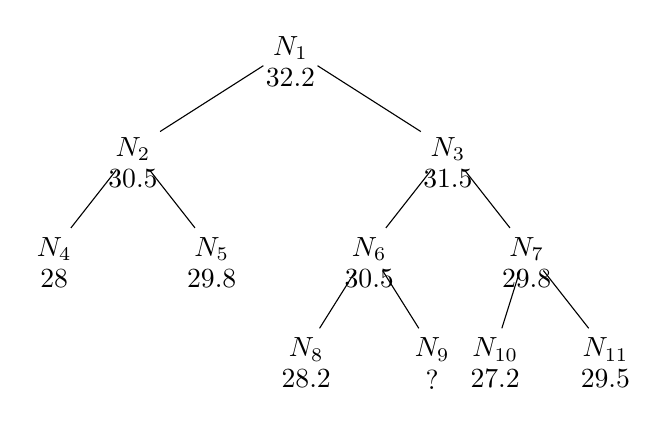
\begin{tikzpicture}[x=1cm,y=.85cm]
\foreach \n/\x/\y/\v in {1/0/0/32.2,2/-2/-1.5/30.5,3/2/-1.5/31.5,4/-3/-3/28,5/-1/-3/29.8,6/1/-3/30.5,7/3/-3/29.8,8/.2/-4.5/28.2,9/1.8/-4.5/?,10/2.6/-4.5/27.2,11/4/-4.5/29.5}{\node(\n)at(\x,\y){$N_{\n}$};\node[below]at(\x,\y-.16){$\v$};}
\foreach \a/\b in {1/2,1/3,2/4,2/5,3/6,3/7,6/8,6/9,7/10,7/11}{\draw(\a)--(\b);}
\end{tikzpicture}\end{center}
(a) $N_9$ 松弛值 $v_9$ 的最佳已知断言是哪项: (i) $v_9\le28.2$; (ii) $v_9=30.5$; (iii) $v_9\le30.5$; (iv) $v_9\ge28$?
(b) 给整数最优值的最佳上下界.
(c) 给 $N_4,N_5,N_8,N_{10},N_{11}$ 各标活跃 A、已剪 F、或信息不足 NEI.
\end{exercise}
\begin{solution}
官方解答重构. (a) 选(iii), 子节点松弛集合包含于父 $N_6$ 松弛集; 不与兄弟 $N_8$ 的28.2比较. (b) 下界28来自已知整数方案. 尚可能改善的叶子 $N_5,N_9,N_{11}$ 中, 最大已知松弛上界30.5, 整数目标向下取整得上界30, 所以 $28\le v^*\le30$. (c) 依次 F、A、F、F、A. $N_4$ 已整数; $N_8$ 的整数目标至多 $\lfloor28.2\rfloor=28$, $N_{10}$ 至多27, 都不能改善; $N_5,N_{11}$ 的非整数松弛值大于28, 按当前信息需保留. 不把非整数 LP 点本身用作整数当前最好值.
\end{solution}

\begin{exercise}\label{ass:15053-practice-q5b}
原题5(b), 第二个 Problem 5, 原标题 Gomory Cut. 纯整数规划的最优松弛表有五个变量列 $x_1,x_2,x_3,x_4,x_5$, 最后一列为 RHS:
\[
\begin{pmatrix}0&0&-2.4&-0.25&0&-26.6\\1&0&2.65&-0.2&0&3.3\\0&1&0.24&0.4&0&4.5\\0&0&0.3&-4.3&1&0.9\end{pmatrix},
\]
全部变量非负. 从第一条\textbf{约束行}推导 Gomory 割, 给步骤.
\end{exercise}
\begin{solution}
官方方法重构, AI 修正最终变量名称. 第一约束 $x_1+2.65x_3-0.2x_4=3.3$. 系数向下取整给 $x_1+2x_3-x_4\le3$. 与原等式相减, 得
$0.65x_3+0.8x_4\ge0.3$. 注意 $\lfloor-0.2\rfloor=-1$, 其分数部分为0.8. 官方末式写成 $0.65x_2+0.8x_3\ge0.3$, 变量错位; 这里从给定行直接计算, 不采用误植. 当前基本解 $x_3=x_4=0$ 违反该割, 而所有非负整数可行点满足.
\end{solution}
